%% Chapter 7 : Generation Forecasting using ARIMA

\section{Introduction to Time Series Analysis}
\
\
\
\
Time series of data is a time ordered sequence of data-points of a particular variable. The data-points in a time series are measured/recorded/logged at successive equally spaced points in time. The time series analysis consists of methods to extract meaningful statistical and other characteristic of the data. Forecasting and Regression are two different methods employed in time series analyses;  where forecasting is concerned with developing a model which can predict future values of time series based on its previous values, and regression is concerned with developing models which give relationships between  current values of one or time series.\\

The application of time series has a large spectrum of areas, some of the are listed below:

\begin{itemize}

\item Statistics

\item Signal Processing and Communication Engineering

\item Econometrics and Mathematical Finance

\item Weather Forecasting and Earthquake Prediction

\end{itemize} 

\section{Time Series Models}
\
\
\
\
There are primarily four time series forecasting models based on the conditional mean and stationarity assumption : AR, MA, ARMA and ARIMA which are discusse in the following sections.

\subsection{AR Model}
\
\
\
\
The AR model is Auto-Regressive Model. It models a certain time-varying univariate data series such that its outputs depend linearly on its own previous values and on a stochastic term. It is a special case of the ARMA and ARIMA models. Also, it can have a unit root (that is the series becomes stationary after taking one difference) i.e. it is not always stationary. The eq (\ref{AR1},\ref{AR2},\ref{AR3},\ref{AR4}) describe the AR Model.

\begin{equation}
\label{AR1}
y_{t} = c + \Phi_{1}y_{t-1} + ... + \Phi_{p}y_{t-p} + \varepsilon_{t^{'}}
\end{equation}\\
where,\\
$ y_{t} $ = Univariate Data Series \\
$ c $ = Model Constant  \\ 
$ \varepsilon_{t^{'}} $ = Unpredictable Part of the Series  \\ 

\begin{equation}
\label{AR2}
L^{i}y_{t} = y_{t-i}
\end{equation}\\
$ L^{i} $ = Lagged Operator of Degree $ i $


\begin{equation}
\label{AR3}
\Phi(L) = ( 1 - \Phi_{1}L - ... - \Phi_{p}L^{p} )
\end{equation}\\
where,\\
$ \Phi(L) $ = Lag Operator Polynomial of the AR Process\\

\begin{equation}
\label{AR4}
\Phi(L)y_{t} = c + \varepsilon_{t^{'}}
\end{equation}

The Fig (\ref{figc7h1}) illustrates a time series of a data variable which can be modeled as an AR process.

\begin{figure}[H]
\centering
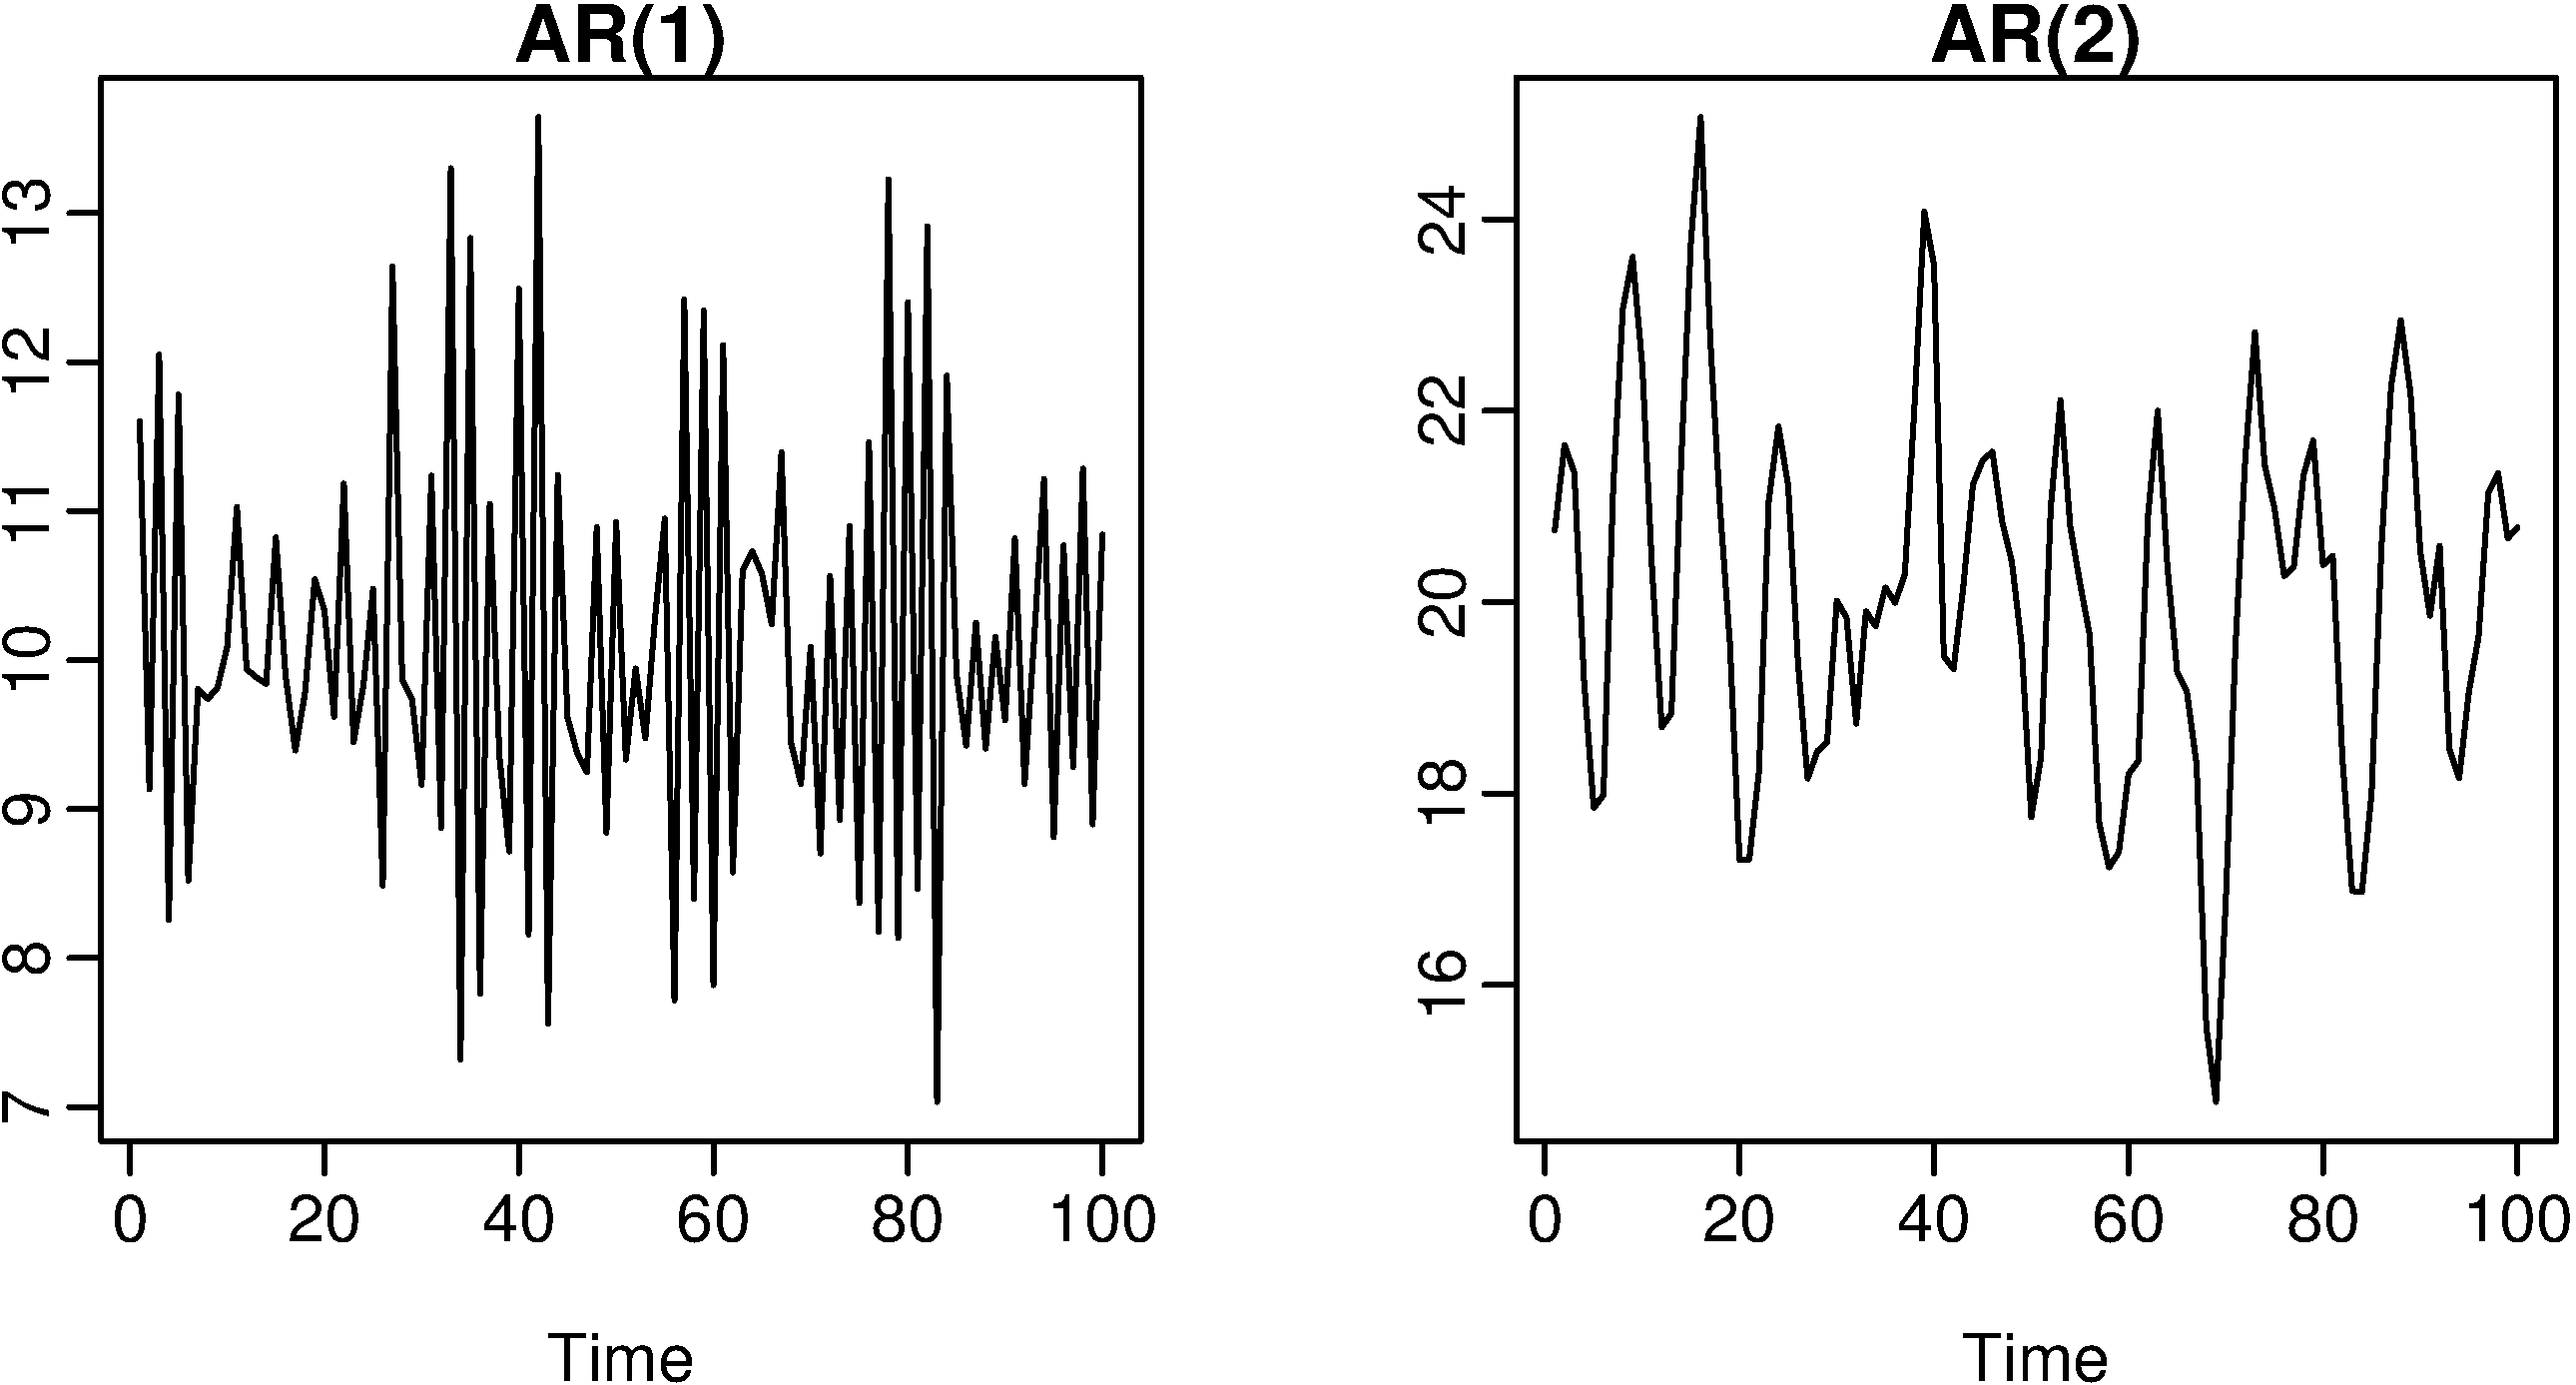
\includegraphics[scale=0.1]{ARIMAImg1}
\caption{An Data Series with AR Process}
\label{figc7h1} %% to refer use, \ref{}
\end{figure}

\subsection{MA Model}
\
\
\
\
The MA model is Moving Average Model.It models a certain time-varying univariate data series such that its outputs depend linearly on the current and previous values of the stochastic term. It is a special case of the ARMA and ARIMA models.
The eq (\ref{MA1},\ref{MA2},\ref{MA3}) describe the MA Model.

\begin{equation}
\label{MA1}
y_{t}= c + \varepsilon_{t} + \theta_{1}\varepsilon_{t-1} + ... + \theta_{q}\varepsilon_{t-q^{'}}
\end{equation}\\
where,\\
$ \varepsilon_{t}, varepsilon_{t-q} $ = Current and past errors of the series \\
 

\begin{equation}
\label{MA2}
\theta(L) = ( 1 + \theta_{1}L + ... + \theta_{p}L^{p} )
\end{equation}\\
where,\\
$ \theta(L) $ = Lag Operator Polynomial of the MA Process\\

\begin{equation}
\label{MA3}
y_{t} = \mu + \theta\varepsilon_{t^{'}}
\end{equation}\\
$ \mu $ = It is the unconditional mean of the MA process

The Fig (\ref{figc7h2}) illustrates a time series of a data variable which can be modeled as an MA process.

\begin{figure}[H]
\centering
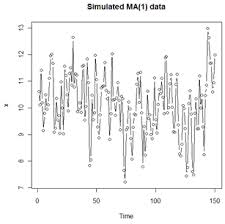
\includegraphics[scale=1]{ARIMAImg2}
\caption{An Data Series with MA Process}
\label{figc7h2} %% to refer use, \ref{}
\end{figure}

\subsection{ARMA Model}
\
\
\
\
The ARMA model is the Auto-Regressive Moving Average Model. It consists of both the AR and the MA part. It is used to model more complex univariate data series. Hence, the output of the ARMA model depends on both the previous data values, and the current and previous stochastic term. AR and MA models are its special case.
The eq (\ref{ARMA1},\ref{ARMA2}) describe the ARMA Model.

\begin{equation}
\label{ARMA1}
y_{t}= c + \Phi_{1}y_{t-1} + ... + \Phi_{p}y_{t-p} + \varepsilon_{t} +  \theta_{1}\varepsilon_{t-1} + ... + \theta_{q}\varepsilon_{t-q^{'}}
\end{equation}\\


\begin{equation}
\label{ARMA2}
\Phi(L)y_{t} = c + \theta\varepsilon_{t^{'}}
\end{equation}\\

The Fig (\ref{figc7h3}) illustrates a time series of a data variable which can be modeled as an ARMA process.

\begin{figure}[H]
\centering
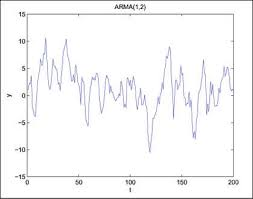
\includegraphics[scale=1]{ARIMAImg3}
\caption{An Data Series with ARMA Process}
\label{figc7h3} %% to refer use, \ref{}
\end{figure}

\subsection{ARIMA Model}
\
\
\
\
The ARIMA model is the Auto-Regressive Moving Average Model. it is a generalization of the ARMA model, and it can model even non-stationary univariate data series by means of using differencing to convert non-stationary series to stationary series. It consists of both the AR and the MA part similar to the ARMA model. Hence, the output of the ARIMA model depends on both the previous data values, and the current and previous stochastic term. ARMA, AR and MA models are its special case.
The eq (\ref{ARIMA1},\ref{ARIMA2}) describe the ARMA Model.

\begin{equation}
\label{ARIMA1}
\bigtriangleup^{D}y_{t}= c + \Phi_{1}\bigtriangleup^{D}y_{t-1} + ... + \Phi_{p}\bigtriangleup^{D}y_{t-p} + \varepsilon_{t} +  \theta_{1}\bigtriangleup^{D}\varepsilon_{t-1} + ... + \theta_{q}\bigtriangleup^{D}\varepsilon_{t-q^{'}}
\end{equation}\\
where,\\
$ \bigtriangleup^{D} $ = It is the difference operator of degree D

\begin{equation}
\label{ARIMA2}
\Phi(L)(1-L^{D})y_{t} = c + \theta\varepsilon_{t^{'}}
\end{equation}\\

The Fig (\ref{figc7h4}) illustrates a time series of a data variable which can be modeled as an ARIMA process.

\begin{figure}[H]
\centering
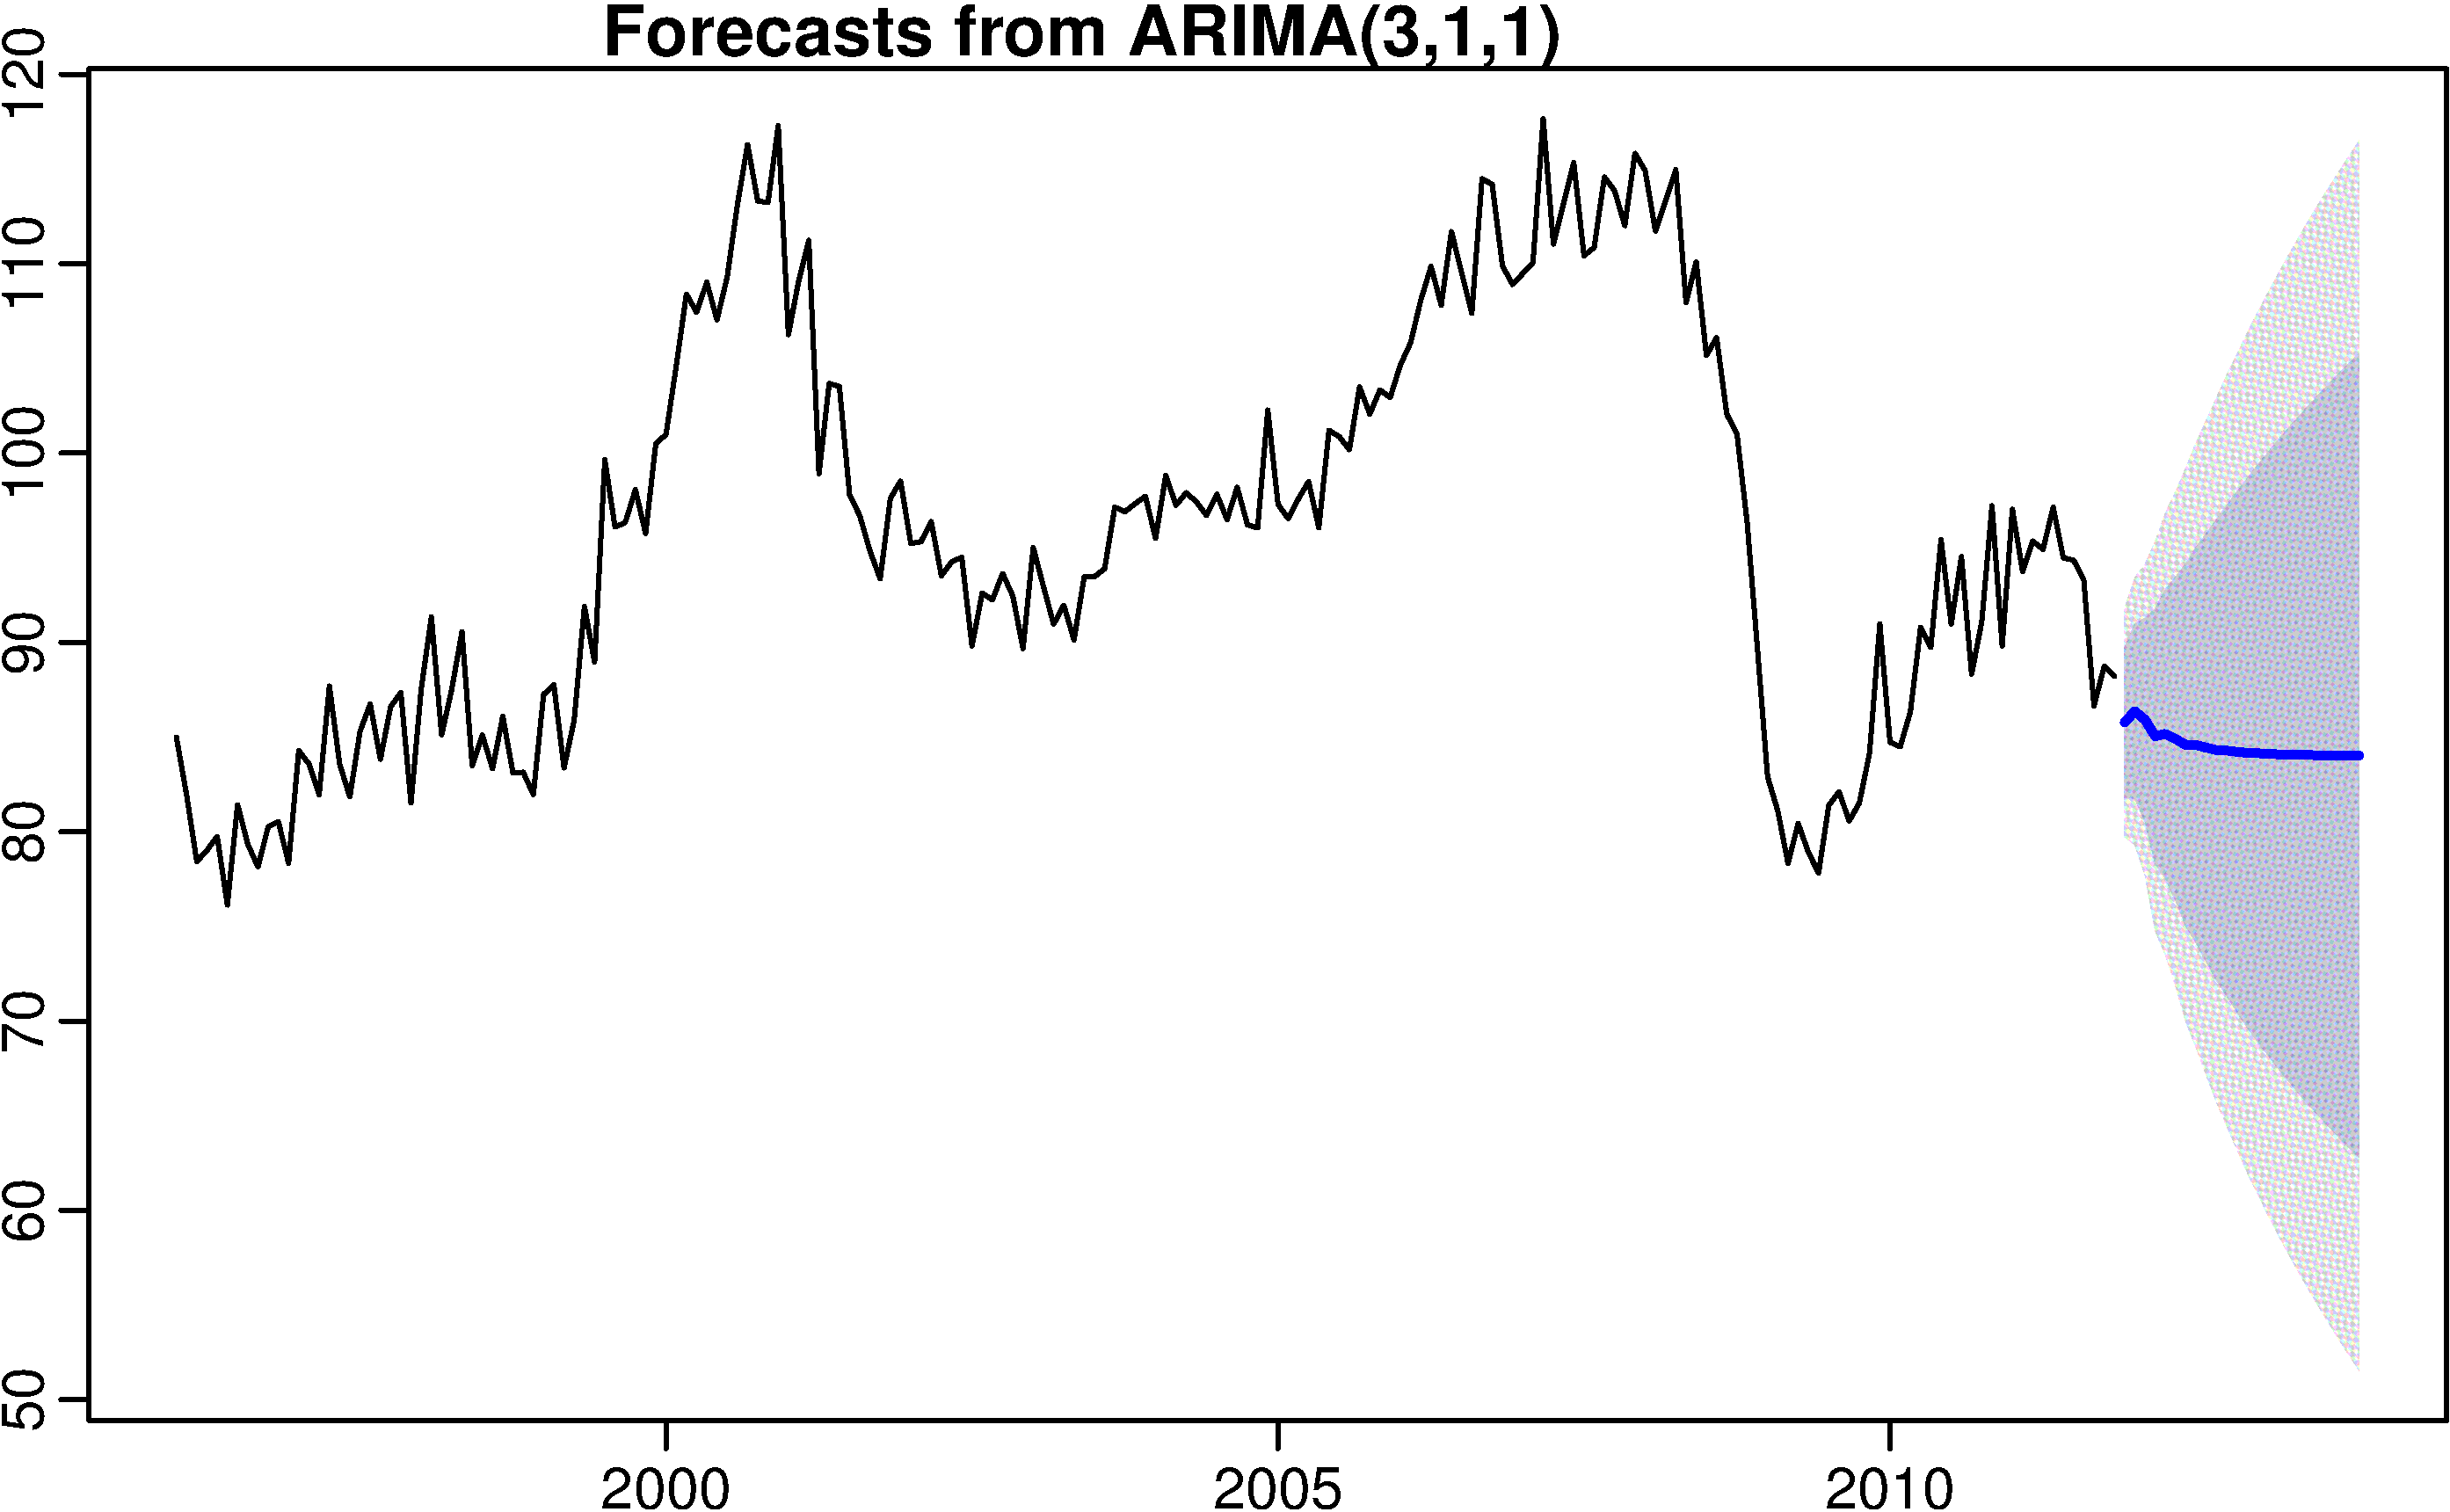
\includegraphics[scale=0.75]{ARIMAImg4}
\caption{An Data Series with ARIMA Process}
\label{figc7h4} %% to refer use, \ref{}
\end{figure}

\section{Model Identification}
\
\
\
\
The first step in time series forecasting is to identify which time series forecasting model described above would best describe the given data series. The concept of Stationarity, the ACF (Auto-Correlation Function), and the PACF (Partial Auto-Correlation Function) helps us in making an intelligent guess for the best model to be used to forecast the given time series data.

\subsection{Concept of Stationarity}
\
\
\
\
The Fig (\ref{figc7h5}) shows a stationary data time series, it can be seen that visually a stationary process seems to be like white noise with no certain pattern whatsoever. If a data time series is stationary the we can rule out ARIMA and focus on ARMA, AR and MA models which could best describe the series.

\begin{figure}[H]
\centering
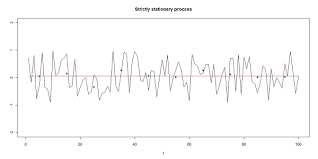
\includegraphics[scale=1]{ARIMAImg5}
\caption{A Stationary Time Series}
\label{figc7h5} %% to refer use, \ref{}
\end{figure}

However, if the data time series is non-stationary i.e. it shows some kind of a pattern as illustrated in the Fig (\ref{figc7h6}), then the series has to be modeled as an ARIMA process.

\begin{figure}[H]
\centering
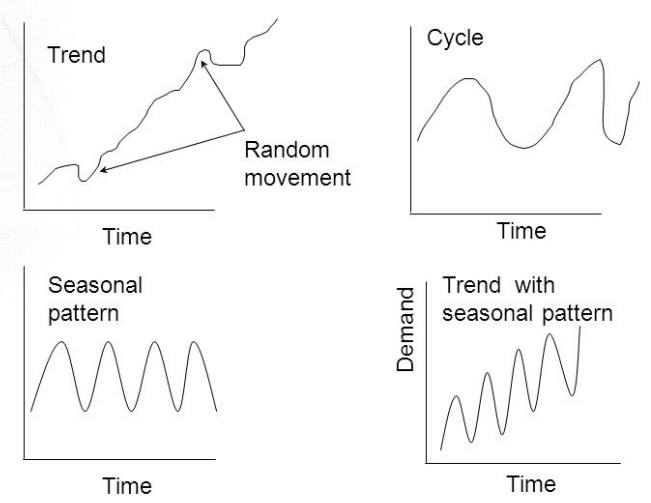
\includegraphics[scale=0.5]{ARIMAImg6}
\caption{Types of Non-Stationary Time Series}
\label{figc7h6} %% to refer use, \ref{}
\end{figure}

The different components of a non-stationary time series are described as follows:

\begin{itemize}

\item \textbf{Trend Component:} A trend exists when there is a long-term increase or decrease in the data. It does not have to be linear. Sometimes we will refer to a trend “changing direction” when it might go from an increasing trend to a decreasing trend. It is illustrated in the Fig (\ref{figc7h6})

\item \textbf{Seasonal Component:} A seasonal pattern exists when a series is influenced by seasonal factors (e.g., the quarter of the year, the month, or day of the week). Seasonality is always of a fixed and known period. It is illustrated in the Fig (\ref{figc7h6})

\item \textbf{Cyclic Component:} A cyclic pattern exists when data exhibit rises and falls that are not of fixed period. The duration of these fluctuations is usually of at least 2 years. It is illustrated in the Fig (\ref{figc7h6})

\end{itemize}

However, real data series may contain one or all of these  components as illustrated in the Fig (\ref{figc7h6}) with a data series having both trend and seasonal pattern.\\

The Dickey-Fuller Test and the Augmented Dickey-Fuller Test are a good measure of stationarity of a time series data.

\subsection{ACF and PACF}
\
\
\
\

Autocorrelation Function (ACF), also known as serial correlation, is the correlation of a signal with itself at different points in time. Informally, it is the similarity between observations as a function of the time lag between them. It is a mathematical tool for finding repeating patterns, such as the presence of a periodic signal obscured by noise, or identifying the missing fundamental frequency in a signal implied by its harmonic frequencies. .\\

The partial autocorrelation function (PACF) gives the partial correlation of a time series with its own lagged values, controlling for the values of the time series at all shorter lags. It contrasts with the autocorrelation function, which does not control for other lags.\\

The Fig (\ref{figc7h7}) shows the ACF and PACF plots for a first order AR and a first order MA process.

\begin{figure}[H]
\centering
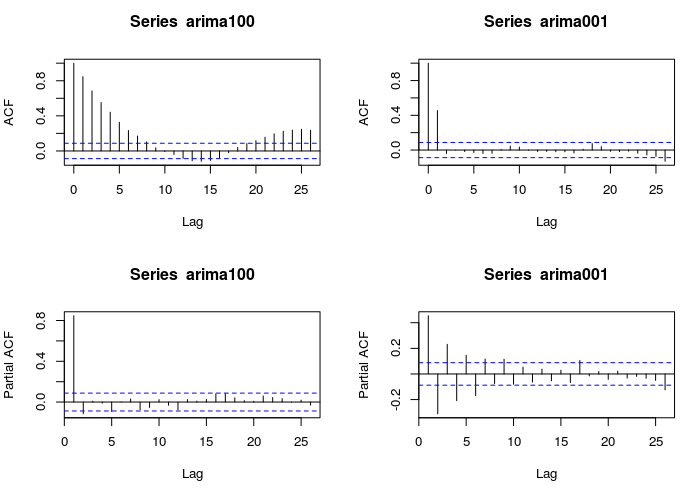
\includegraphics[scale=0.5]{ARIMAImg7}
\caption{ACF and PACF Graphs for AR and MA Processes}
\label{figc7h7} %% to refer use, \ref{}
\end{figure}

Both ACF and PACF are indispensable tools in selection of the best time series model for time series data forecasting. Some basic thumb rules for interpreting the ACF and PACF plots are given in the Table (\ref{ARIMATab1})

\begin{table}[H]
  \centering
  \caption{Nature of ACF and PACF for Different Time Series Models}
    \begin{tabular}{|l|l|l|}
    \hline
    \multicolumn{1}{|c|}{\textbf{Model}} & \multicolumn{1}{c|}{\textbf{ACF}} & \multicolumn{1}{c|}{\textbf{PACF}} \bigstrut\\
    \hline
    AR(p) & Tails off gradually & Cuts off after p lags \bigstrut\\
    \hline
    MA(q) & Cuts off after q lags & Tails off gradually \bigstrut\\
    \hline
    ARMA(p,q) & Tails off gradually & Tails off gradually \bigstrut\\
    \hline
    \end{tabular}%
  \label{ARIMATab1}%
\end{table}%

The Ljung-Box Q Test is an excellent statistical tool to measure the amount of correlation present between different lags of the ACF and PACF plots. It helps us in identifying the time series models more effectively.


\section{Model Estimation and Fitness}
\
\
\
\
After completing the model identification, usually two to three variations of the model identified are created for being more certain of our choice. In estimation of the models the co-efficients of the AR, MA, ARMA and ARIMA model (depending on the forecasters choice) equations are calculated.\\

Using these complete equations, model statistics are computed for each of the estimated model. The standardized residuals are of great importance in determining the best model to be selected for forecasting. For a good estimated model its standardized residuals should represent white noise i.e. there is no correlation whatsoever in the residuals. Further more the AIC (Akalike Information Criterion) and the BIC (Bayesian Information Criterion) are quantitative measure for better model estimation, the model with least AIC and BIC values is the best esitmated model.\\

Once the decision is made using above criteria, the best model is then used for forecasting the time series data.\\




\section{Process Flow for Forecasting using ARIMA Model}
\
\
\
\
The Fig (\ref{figc7ARIMAFlow}) shows the schematic of the process flow for the development of the ARIMA model for forecasting.

\begin{figure}[H]
\centering
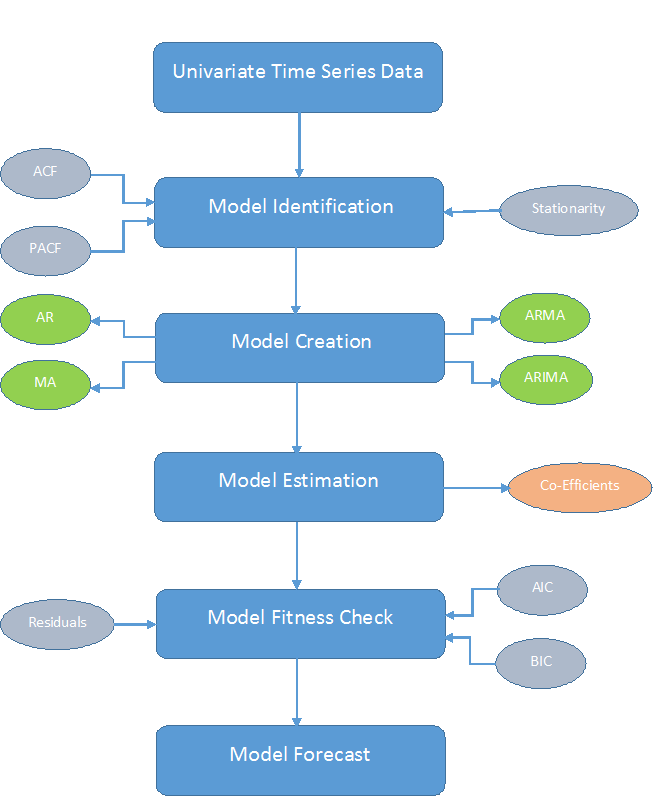
\includegraphics[scale=0.8]{ARIMA_Flow}
\caption{Schematic of ARIMA Model Development for Forecasting}
\label{figc7ARIMAFlow} %% to refer use, \ref{}
\end{figure}

\section{Results}
\
\
\
\
The results for generation forecasting using ARIMA have been produced for the GSEC 1MW SPVP. The data utisiled for estimating the ARIMA coefficients is the WRF weather variables generated for the same plant for the month of June 2016 (The WRF results will be discussed in Chapter 9). The forecasted weather variables form the ARIMA models have been fed as inputs to the solar energy estimation app to generate the intra-hour generation forecast.\\

\subsection{GSEC 1MW SPVP - Plant Information}
\
\
\
\
The Table (\ref{AnnAppTab1}) gives the site and PV module information of the GSEC 1MW SPVP.

\begin{table}[H]
  \centering
  \caption{GSEC 1MW SPVP Plant Information Table}
    \begin{tabular}{|l|c|c|c|c|c|}
    \hline
    \multicolumn{6}{|c|}{\textbf{GSEC 1MW SVPP}} \bigstrut\\
    \hline
    \multicolumn{6}{|c|}{\textbf{SITE INFORMATION}} \bigstrut\\
    \hline
    \textbf{LATITUDE} & \multicolumn{5}{c|}{23.275} \bigstrut\\
    \hline
    \textbf{LONGITUDE} & \multicolumn{5}{c|}{72.682} \bigstrut\\
    \hline
    \textbf{PLANT CAPACITY (MW)} & \multicolumn{5}{c|}{1} \bigstrut\\
    \hline
    \multicolumn{6}{|c|}{\textbf{PV MODULE INFORMATION}} \bigstrut\\
    \hline
    \textbf{DESCRIPTION} & A-si & Cdte & Cigs & Multi & Mono \bigstrut\\
    \hline
    \textbf{MAKE} & Du-Pont & First Solar & Q Cells & Lanco & Lanco \bigstrut\\
    \hline
    \textbf{CRYSTALLINE/THIN-FILM} & Thin-Film & Thin-Film & Thin-Film & Crystalline & Crystalline \bigstrut\\
    \hline
    \textbf{RATING (W)} & 107 & 85 & 95 & 235 & 250 \bigstrut\\
    \hline
    \textbf{Vmpp (V)} & 74 & 46.4 & 62.1 & 29.56 & 31.15 \bigstrut\\
    \hline
    \textbf{Impp (A)} & 1.44 & 1.83 & 1.53 & 7.95 & 8.034 \bigstrut\\
    \hline
    \textbf{Voc (V)} & 99 & 60.5 & 78 & 37.17 & 38.04 \bigstrut\\
    \hline
    \textbf{Isc (A)} & 1.81 & 1.94 & 1.68 & 8.4 & 8.712 \bigstrut\\
    \hline
    \textbf{TEMP COEFF OF Voc} & -0.3 & -0.27 & -0.29 & -0.31 & -0.33 \bigstrut\\
    \hline
    \textbf{TEMP COEFF OF Isc} & 0.09 & 0.04 & 0.04 & 0.06 & 0.036 \bigstrut\\
    \hline
    \textbf{TEMP COEFF OF Pmp} & -0.25 & -0.25 & -0.38 & -0.43 & -0.47 \bigstrut\\
    \hline
    \textbf{TOTAL MODULES} & 924 & 1170 & 1056 & 432 & 405 \bigstrut\\
    \hline
    \textbf{LENGTH (mm)} & 1436 & 1200 & 1196 & 1360 & 1360 \bigstrut\\
    \hline
    \textbf{BREADTH (mm)} & 1117 & 600 & 636 & 941 & 951 \bigstrut\\
    \hline
    \textbf{AREA (m2)} & 1.604012 & 0.72 & 0.760656 & 1.27976 & 1.29336 \bigstrut\\
    \hline
    \end{tabular}%
  \label{AnnAppTab1}%
\end{table}%

\subsection{ARIMA Results}
\
\
\
\
The ARIMA weather variable forecasted outputs using ARIMA models in comparison with the original data series used are given in the Fig (\ref{figc7ARIMAWs},\ref{figc7ARIMAT},\ref{figc7ARIMAIr}).

\begin{figure}[H]
\centering
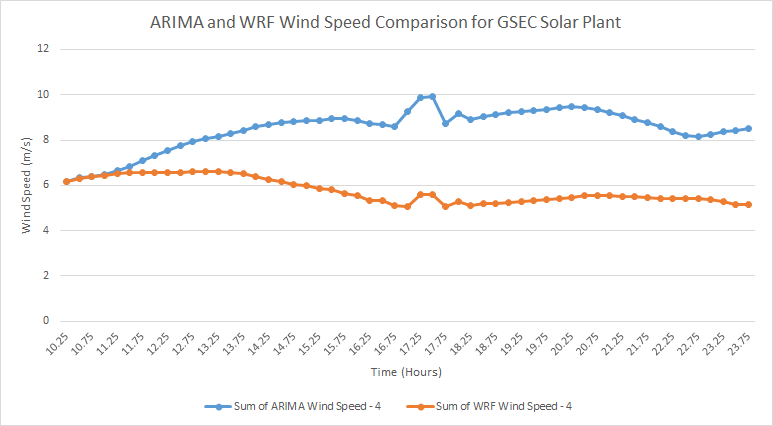
\includegraphics[scale=0.8]{ARIMA_Ws}
\caption{Comparison of Wind Speed Prediction using ARIMA with Original Data Series obtained from WRF }
\label{figc7ARIMAWs} %% to refer use, \ref{}
\end{figure}

\begin{figure}[H]
\centering
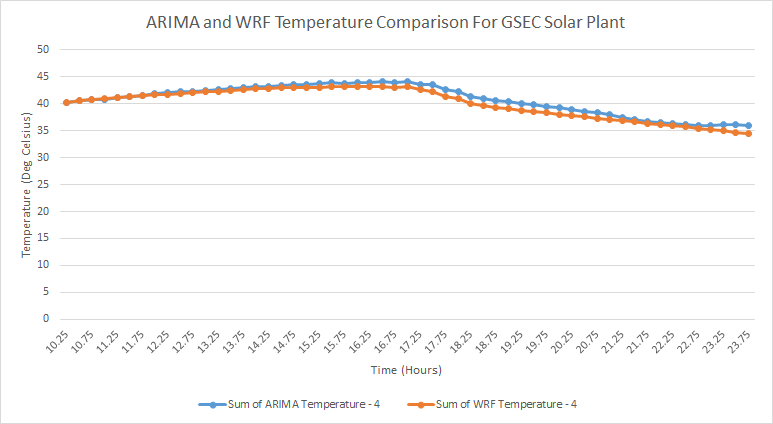
\includegraphics[scale=0.8]{ARIMA_T}
\caption{Comparison of Temperature Prediction using ARIMA with Original Data Series obtained from WRF }
\label{figc7ARIMAT} %% to refer use, \ref{}
\end{figure}

\begin{figure}[H]
\centering
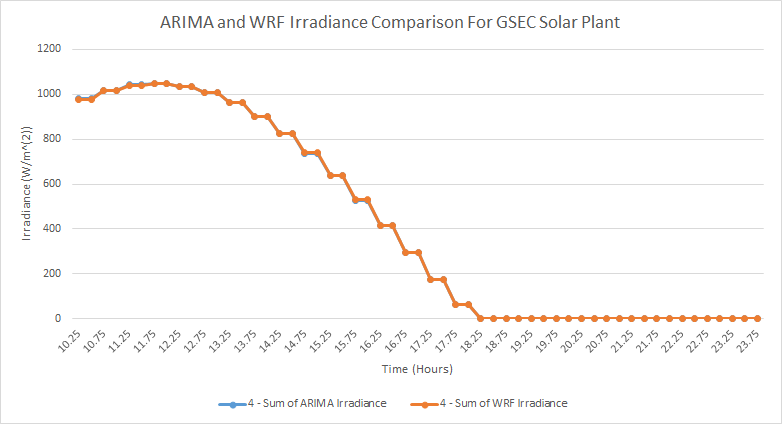
\includegraphics[scale=0.8]{ARIMA_Ir}
\caption{Comparison of Irradiance Prediction using ARIMA with Original Data Series obtained from WRF }
\label{figc7ARIMAIr} %% to refer use, \ref{}
\end{figure}

The energy generation forecast for the GSEC plant is computed using the ARIMA forecasted weather variables using the solar energy estimation application. The forecast is generated from 10.25 (Decimal Time), $4^{th}$ June, 2016 to 10.00 (Decimal Time), $5^{th}$ June, 2016. The weather data series of WRF used are from 0.00 (Decimal Time), $1^{st}$ June, 2016 to 10.00 (Decimal Time), $4^{th}$ June, 2016.

\begin{figure}[H]
\centering
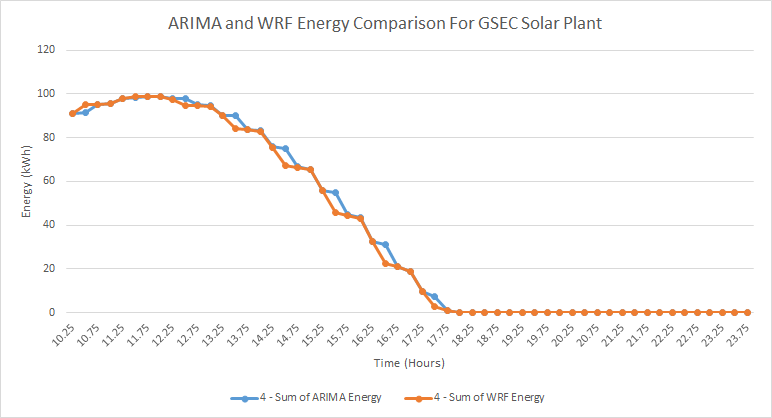
\includegraphics[scale=0.8]{ARIMA_En}
\caption{Comparison of Energy Prediction using ARIMA with Original Data Series obtained from WRF }
\label{figc7ARIMAEn} %% to refer use, \ref{}
\end{figure}

\newpage

\subsection{Conclusion from Graphs}

All the ARIMA models used are of seasonal type with seasonality of 96 as the data series has a resolution of 15 minutes. Moreover, it has been observed that the ARIMA models with both AR and MA components forecast better. All the original data series have been differenced twice. From the Fig (\ref{figc7ARIMAWs},\ref{figc7ARIMAT},\ref{figc7ARIMAIr},\ref{figc7ARIMAEn}), we see that the ARIMA models have been able to predict the weather variables and the energy output with a good degree of accuracy.
